% ============================================================
% SECTION 10.6 & 10.7: PREFERENCE-BASED SETTING & OTHER RANKING CRITERIA
% Thành viên 3 - Biên soạn dựa trên Chương 10: Foundations of Machine Learning (Mohri, 2018)
% ============================================================

% ============================================================
\subsection{Cách Tiếp Cận Dựa Trên Ưu Tiên (Preference-Based Setting)}
\label{sec:preference}

\subsubsection{Động Lực và So Sánh Với Score-Based Setting}

Trong phần trước, chúng ta đã nghiên cứu \emph{score-based setting}: thuật toán học một hàm cho điểm toàn cục $h : \mathcal{X} \to \mathbb{R}$, trong đó thứ hạng của mọi phần tử $x \in \mathcal{X}$ được xác định hoàn toàn bởi điểm số $h(x)$. Cách tiếp cận này có một hạn chế cơ bản: vì $h$ cảm sinh một thứ tự tuyến tính \emph{bắc cầu} trên $\mathcal{X}$, nó không thể biểu diễn chính xác khi hàm ưu tiên thực sự $f$ \emph{không bắc cầu} (ví dụ: ưu tiên theo vòng tròn $f(u,v)=1$, $f(v,w)=1$, $f(w,u)=1$).

\textbf{Cách tiếp cận preference-based} (dựa trên ưu tiên) giải quyết hạn chế này bằng cách thay đổi mục tiêu:
\begin{itemize}
    \item Thay vì cần xếp hạng toàn bộ không gian $\mathcal{X}$, ta chỉ cần xếp hạng chính xác một \emph{tập con truy vấn hữu hạn} (finite query subset) $X \subseteq \mathcal{X}$ tại thời điểm kiểm tra.
    \item Hàm ưu tiên $h : \mathcal{X} \times \mathcal{X} \to [0,1]$ \emph{không bắt buộc phải bắc cầu}: ta có thể có $h(u,v) = h(v,w) = h(w,u) = 1$ cho ba điểm phân biệt $u, v, w$.
\end{itemize}

Thiết lập này rất tự nhiên trong các ứng dụng như \textbf{search engine} (xếp hạng kết quả cho một truy vấn cụ thể), \textbf{hệ thống khuyến nghị} (xếp hạng danh sách phim cho từng người dùng), hay \textbf{fraud detection} (xếp hạng giao dịch đáng ngờ nhất trong một đợt kiểm tra).

\begin{table}[h]
\centering
\small
\begin{tabular}{lll}
\hline
\textbf{Đặc điểm} & \textbf{Score-based} & \textbf{Preference-based} \\
\hline
Đầu ra học & Hàm điểm $h:\mathcal{X}\to\mathbb{R}$ & Hàm ưu tiên $h:\mathcal{X}\times\mathcal{X}\to[0,1]$ \\
Tính bắc cầu & Bắt buộc (do dùng điểm số) & Không bắt buộc \\
Phạm vi xếp hạng & Toàn bộ $\mathcal{X}$ & Tập con truy vấn $X \subseteq \mathcal{X}$ \\
Liên hệ với phân loại & Gián tiếp & Trực tiếp (quy về classification) \\
\hline
\end{tabular}
\caption{So sánh score-based và preference-based setting.}
\label{tab:pref_vs_score}
\end{table}

% -------- 10.6.1  Bài toán giai đoạn thứ hai --------
\subsubsection{Hai Giai Đoạn Của Preference-Based Setting}

Preference-based setting được chia thành \textbf{hai giai đoạn} tách biệt:

\paragraph{Giai đoạn 1: Học hàm ưu tiên}
Sử dụng tập mẫu huấn luyện $S = \{(x_1, x'_1, y_1), \ldots, (x_m, x'_m, y_m)\}$ với $y_i \in \{-1, 0, +1\}$, ta học một \textbf{hàm ưu tiên} $h : \mathcal{X} \times \mathcal{X} \to [0,1]$ sao cho:
\begin{itemize}
    \item $h(u, v) \approx 1$: $u$ được ưu tiên hơn $v$ (nên xếp trên $v$).
    \item $h(u, v) \approx 0$: $v$ được ưu tiên hơn $u$.
    \item Điều kiện nhất quán theo cặp: $h(u,v) + h(v,u) = 1$ với mọi $u, v \in \mathcal{X}$.
\end{itemize}

Hàm $h$ có thể được học bởi \emph{bất kỳ thuật toán phân loại nhị phân nào}, ví dụ SVM với $h(u,v) = \sigma(\mathbf{w}^\top(\phi(u) - \phi(v)))$ hoặc một mạng nơ-ron.

\paragraph{Giai đoạn 2: Xếp hạng tập con truy vấn}
Cho tập con truy vấn $X \subseteq \mathcal{X}$ (hữu hạn), sử dụng hàm $h$ đã học để sinh ra một thứ hạng $\sigma: X \to \{1, \ldots, |X|\}$ sao cho sai lệch so với thứ hạng đích $\sigma^*$ là nhỏ nhất. Đây là trọng tâm lý thuyết của phần này.

\begin{definition}[Hàm ưu tiên nhất quán theo cặp]
Một hàm $h: \mathcal{X} \times \mathcal{X} \to [0,1]$ được gọi là \textbf{nhất quán theo cặp} (pairwise consistent) nếu với mọi $u, v \in \mathcal{X}$:
\begin{equation}
    h(u, v) + h(v, u) = 1.
    \label{eq:pairwise_consistent}
\end{equation}
\end{definition}

Điều kiện \eqref{eq:pairwise_consistent} đảm bảo rằng nếu $h$ nói ``$u$ được ưu tiên hơn $v$ với xác suất $p$'', thì đồng thời nó nói ``$v$ được ưu tiên hơn $u$ với xác suất $1-p$''. Đây là điều kiện tối thiểu về tính nhất quán cho một hàm ưu tiên.

% -------- Mô hình xác suất --------
\subsubsection{Mô Hình Xác Suất Cho Bài Toán Giai Đoạn Thứ Hai}

Bài toán giai đoạn thứ hai được mô hình hóa theo khuôn khổ xác suất như sau. Gọi $\mathcal{D}$ là một phân phối ẩn trên các cặp $(X, \sigma^*)$, trong đó:
\begin{itemize}
    \item $X \subseteq \mathcal{X}$ là tập con truy vấn (query subset) hữu hạn,
    \item $\sigma^*: X \to \{1, \ldots, |X|\}$ là thứ hạng mục tiêu (target ranking), tức là một song ánh từ $X$ vào $\{1, \ldots, |X|\}$.
\end{itemize}

Một thuật toán $\mathcal{A}$ nhận đầu vào là $X$ và hàm ưu tiên $h$ (đã học ở giai đoạn 1), và trả về một thứ hạng $\mathcal{A}(X)$ của $X$. Thuật toán có thể là \emph{xác định} (deterministic) hoặc \emph{ngẫu nhiên} (randomized), trong trường hợp sau ta ký hiệu seed ngẫu nhiên là $s$.

% -------- Hàm mất mát --------
\subsubsection{Hàm Mất Mát Và Regret}
\label{sec:pref_loss}

Để đo mức độ sai lệch giữa thứ hạng dự đoán $\sigma$ và thứ hạng mục tiêu $\sigma^*$ trên tập $X$ có $n \geq 1$ phần tử, giáo trình định nghĩa:

\begin{definition}[Hàm mất mát xếp hạng cặp]
\begin{equation}
    L(\sigma, \sigma^*) = \frac{2}{n(n-1)} \sum_{u \neq v} \mathbf{1}_{\sigma(u) < \sigma(v)}\, \mathbf{1}_{\sigma^*(v) < \sigma^*(u)},
    \label{eq:loss_pref}
\end{equation}
trong đó tổng chạy qua tất cả các cặp $(u, v)$ phân biệt trong $X$.
\end{definition}

\textbf{Giải thích trực quan:} $\sigma(u) < \sigma(v)$ nghĩa là $\sigma$ đặt $u$ xếp trước $v$ (vị trí thấp hơn = xếp cao hơn). Cặp $(u,v)$ đóng góp vào mất mát khi $\sigma$ xếp $u$ trước $v$, nhưng $\sigma^*$ lại xếp $v$ trước $u$, tức là \emph{xếp sai}. Hệ số $\frac{2}{n(n-1)}$ chuẩn hóa để $L \in [0,1]$.

\begin{example}[Tính hàm mất mát bằng tay]
Cho $X = \{a, b, c\}$ với $n=3$. Thứ hạng mục tiêu $\sigma^*$: $a \succ b \succ c$ (tức $\sigma^*(a)=1, \sigma^*(b)=2, \sigma^*(c)=3$). Thứ hạng dự đoán $\sigma$: $b \succ a \succ c$ (tức $\sigma(b)=1, \sigma(a)=2, \sigma(c)=3$).

Ta liệt kê 3 cặp phân biệt và kiểm tra từng cặp:
\begin{enumerate}
    \item Cặp $(a,b)$: $\sigma(a)=2 > \sigma(b)=1$ nên $\sigma(a) < \sigma(b)$ là \textbf{sai} (không thỏa $\sigma(a)<\sigma(b)$). Term = 0.

    Thực ra với cặp này: $\sigma(b)=1 < \sigma(a)=2$, tức $\sigma$ xếp $b$ trước $a$. Còn $\sigma^*(a)=1 < \sigma^*(b)=2$ nên $\sigma^*$ xếp $a$ trước $b$. Vậy $\sigma$ xếp $b$ trước $a$ nhưng $\sigma^*$ xếp $a$ trước $b$ $\Rightarrow$ \textbf{sai}. Đóng góp: $\mathbf{1}_{\sigma(b)<\sigma(a)} \cdot \mathbf{1}_{\sigma^*(a)<\sigma^*(b)} = 1 \cdot 1 = 1$.

    \item Cặp $(a,c)$: $\sigma(a)=2 < \sigma(c)=3$ nên $\sigma$ xếp $a$ trước $c$. $\sigma^*(a)=1 < \sigma^*(c)=3$ nên $\sigma^*$ cũng xếp $a$ trước $c$. $\Rightarrow$ \textbf{đúng}. Đóng góp: 0.

    \item Cặp $(b,c)$: $\sigma(b)=1 < \sigma(c)=3$ nên $\sigma$ xếp $b$ trước $c$. $\sigma^*(b)=2 < \sigma^*(c)=3$ nên $\sigma^*$ cũng xếp $b$ trước $c$. $\Rightarrow$ \textbf{đúng}. Đóng góp: 0.
\end{enumerate}

Chỉ có 1 cặp sai trong 3 cặp, nên:
\[
    L(\sigma, \sigma^*) = \frac{2}{3 \cdot 2} \cdot 1 = \frac{1}{3} \approx 0.333.
\]
\end{example}

\paragraph{Hàm mất mát của hàm ưu tiên $h$.} Tương tự, mất mát của hàm ưu tiên $h$ đối với thứ hạng mục tiêu $\sigma^*$ trên tập $X$ là:
\begin{equation}
    L(h, \sigma^*) = \frac{2}{n(n-1)} \sum_{u \neq v} h(u, v)\, \mathbf{1}_{\sigma^*(v) < \sigma^*(u)}.
    \label{eq:loss_pref_h}
\end{equation}

Ý tưởng: $h$ gây lỗi khi nó cho điểm cao $h(u,v) \approx 1$ (tức nói $u$ được ưu tiên hơn $v$) nhưng thực tế $\sigma^*$ lại xếp $v$ trước $u$ (tức $\sigma^*(v) < \sigma^*(u)$).

\paragraph{Regret của thuật toán và của hàm ưu tiên.}
\begin{definition}[Regret]
\emph{Regret} của một thuật toán xác định $\mathcal{A}$ là:
\begin{equation}
    \mathrm{Reg}(\mathcal{A}) = \mathbb{E}_{(X, \sigma^*) \sim \mathcal{D}}\bigl[L(\mathcal{A}(X), \sigma^*)\bigr] - \min_{\sigma'} \mathbb{E}_{(X, \sigma^*) \sim \mathcal{D}}\bigl[L(\sigma'|_X, \sigma^*)\bigr],
    \label{eq:regret_algo}
\end{equation}
trong đó $\sigma'|_X$ là thứ hạng cảm sinh trên $X$ bởi thứ hạng toàn cục $\sigma'$ trên $\mathcal{X}$.

\emph{Regret} của hàm ưu tiên $h$ là:
\begin{equation}
    \mathrm{Reg}(h) = \mathbb{E}_{(X, \sigma^*) \sim \mathcal{D}}\bigl[L(h|_X, \sigma^*)\bigr] - \min_{h'} \mathbb{E}_{(X, \sigma^*) \sim \mathcal{D}}\bigl[L(h'|_X, \sigma^*)\bigr],
    \label{eq:regret_h}
\end{equation}
trong đó $h|_X$ là hạn chế của $h$ vào $X \times X$.
\end{definition}

Regret đo lường \emph{sự chênh lệch hiệu năng} giữa thuật toán (hoặc hàm ưu tiên) đang xét với cách xếp hạng tốt nhất có thể. Regret nhỏ nghĩa là thuật toán gần với tối ưu.

\paragraph{Giả định PIIA (Pairwise Independence on Irrelevant Alternatives).}
Các kết quả trong phần này giả định tính chất sau:
\begin{equation}
    \mathbb{E}_{\sigma^* | X_1}\bigl[\mathbf{1}_{\sigma^*(v) < \sigma^*(u)}\bigr] = \mathbb{E}_{\sigma^* | X_2}\bigl[\mathbf{1}_{\sigma^*(v) < \sigma^*(u)}\bigr],
    \label{eq:piia}
\end{equation}
với mọi $u, v \in X$ và mọi hai tập $X_1, X_2$ đều chứa $u$ và $v$.

Nghĩa là: xác suất $u$ được ưu tiên hơn $v$ trong thứ hạng mục tiêu $\sigma^*$ \emph{không phụ thuộc vào các phần tử khác} trong tập truy vấn, chỉ phụ thuộc vào bản thân $u$ và $v$. Đây là một dạng điều kiện độc lập giúp đơn giản hóa phân tích lý thuyết.

% -------- 10.6.2 Deterministic --------
\subsubsection{Thuật Toán Xác Định: Sort-by-Degree}
\label{sec:sort_by_degree}

\paragraph{Ý tưởng.} Thuật toán xác định tự nhiên nhất dựa trên hàm ưu tiên $h$ là \textbf{sort-by-degree}: xếp hạng mỗi phần tử theo số phần tử khác mà nó được ưu tiên hơn, theo hàm $h$.

\begin{definition}[Degree của một phần tử]
Cho tập $X$ và hàm ưu tiên $h$, \emph{degree} của phần tử $u \in X$ được định nghĩa là:
\begin{equation}
    \mathrm{deg}_h(u) = \sum_{v \in X,\, v \neq u} h(u, v).
    \label{eq:degree}
\end{equation}
\end{definition}

Thuật toán sort-by-degree $\mathcal{A}_{\text{SBD}}$ sắp xếp các phần tử của $X$ theo thứ tự giảm dần của degree:
\[
    \mathcal{A}_{\text{SBD}}(X) = \text{argsort}_{u \in X}\bigl(-\mathrm{deg}_h(u)\bigr).
\]

\begin{example}[Minh họa Sort-by-Degree]
Cho $X = \{u, v, w\}$ và hàm ưu tiên $h$ với các giá trị:
$h(u,v) = 0.7$, $h(v,u) = 0.3$, $h(u,w) = 0.8$, $h(w,u) = 0.2$, $h(v,w) = 0.6$, $h(w,v) = 0.4$.

Tính degree:
\begin{align*}
    \mathrm{deg}_h(u) &= h(u,v) + h(u,w) = 0.7 + 0.8 = 1.5, \\
    \mathrm{deg}_h(v) &= h(v,u) + h(v,w) = 0.3 + 0.6 = 0.9, \\
    \mathrm{deg}_h(w) &= h(w,u) + h(w,v) = 0.2 + 0.4 = 0.6.
\end{align*}

Xếp hạng theo degree giảm dần: $u \succ v \succ w$, tức $\sigma(u)=1, \sigma(v)=2, \sigma(w)=3$.
\end{example}

\paragraph{Chặn lý thuyết cho Sort-by-Degree.}
\begin{theorem}[Chặn mất mát và regret cho Sort-by-Degree, Section 10.6.2]
\label{thm:sort_by_degree}
Trong cài đặt nhị phân (bipartite), các chặn sau được chứng minh:
\begin{align}
    \mathbb{E}_{X, \sigma^*}\bigl[L\bigl(\mathcal{A}_{\mathrm{SBD}}(X), \sigma^*\bigr)\bigr] &\leq 2\, \mathbb{E}_{X, \sigma^*}\bigl[L(h, \sigma^*)\bigr], \label{eq:sbd_loss} \\
    \mathrm{Reg}\bigl(\mathcal{A}_{\mathrm{SBD}}\bigr) &\leq 2\, \mathrm{Reg}(h). \label{eq:sbd_regret}
\end{align}
\end{theorem}

\begin{proof}[Chứng minh chi tiết]
Chứng minh sử dụng phân tích xác suất trên từng cặp. Ký hiệu $p_{uv}^* = \mathbb{E}_{\sigma^*|X}[\mathbf{1}_{\sigma^*(v) < \sigma^*(u)}]$ là xác suất $v$ được ưu tiên hơn $u$ trong $\sigma^*$.

\textbf{Bước 1: Mất mát của sort-by-degree.}
Thuật toán SBD xếp $u$ trước $v$ khi và chỉ khi $\mathrm{deg}_h(u) > \mathrm{deg}_h(v)$. Xác suất này là:
\[
    \Pr[\mathrm{SBD \ xếp \ } u \text{ trước } v] = \Pr\left[\sum_{w \neq u} h(u,w) > \sum_{w \neq v} h(v,w)\right].
\]

SBD mắc lỗi trên cặp $(u,v)$ khi nó xếp $u$ trước $v$ nhưng $\sigma^*$ xếp $v$ trước $u$. Mất mát kỳ vọng:
\begin{equation}
    \mathbb{E}[L(\mathrm{SBD}, \sigma^*)] = \frac{2}{n(n-1)} \sum_{u \neq v} \Pr[\text{SBD xếp } u \text{ trước } v] \cdot p_{uv}^*.
\end{equation}

\textbf{Bước 2: Chặn trên từ hàm ưu tiên $h$.}
Giả sử $h$ cảm sinh một hàm so sánh bằng cách lấy ngưỡng (ví dụ $h(u,v) > 0.5$ nghĩa là ``$u$ ưu tiên hơn $v$''). Trong cài đặt nhị phân (bipartite), người ta chứng minh rằng:
\begin{align*}
    \Pr[\text{SBD xếp } u \text{ trước } v] &\leq \Pr[\text{hầu hết } w: h(u,w) \geq h(v,w)] \\
    &\leq p_{uv}^* + \mathbb{E}[L(h, \sigma^*)],
\end{align*}
do PIIA và tính nhất quán của $h$.

\textbf{Bước 3: Kết luận.}
Bằng cách tổng hợp trên tất cả các cặp và lấy kỳ vọng theo $(X, \sigma^*)$:
\[
    \mathbb{E}[L(\mathrm{SBD}, \sigma^*)] \leq 2 \mathbb{E}[L(h, \sigma^*)],
\]
which proves \eqref{eq:sbd_loss}. Chặn regret \eqref{eq:sbd_regret} tuân theo định nghĩa.
\end{proof}

\paragraph{Hạn chế của Sort-by-Degree.}
\begin{itemize}
    \item \textbf{Hệ số 2 có thể gây hậu quả nghiêm trọng:} Nếu hàm $h$ chỉ có lỗi 25\%, chặn trong \eqref{eq:sbd_loss} chỉ đảm bảo mất mát xếp hạng không vượt quá 50\%, bằng với xếp hạng ngẫu nhiên!
    \item \textbf{Độ phức tạp bậc hai:} Để tính degree cho mọi phần tử, ta cần gọi $h$ cho \emph{tất cả các cặp} $(u,v)$ trong $X$, dẫn đến độ phức tạp $\Omega(|X|^2)$.
\end{itemize}

% -------- Lower bound --------
\subsubsection{Chặn Dưới Cho Thuật Toán Xác Định (Theorem 10.5)}

Câu hỏi tự nhiên đặt ra là: liệu có thuật toán xác định nào tốt hơn sort-by-degree, với hệ số nhỏ hơn 2? Câu trả lời là \textbf{không}.

\begin{theorem}[Chặn dưới cho thuật toán xác định -- Theorem 10.5]
\label{thm:lower_bound_det}
Với mọi thuật toán xác định $\mathcal{A}$, tồn tại một phân phối bipartite $\mathcal{D}$ sao cho:
\begin{equation}
    \mathrm{Reg}(\mathcal{A}) \geq 2\, \mathrm{Reg}(h).
    \label{eq:lower_bound_det}
\end{equation}
\end{theorem}

\begin{proof}[Chứng minh đầy đủ]
Xét trường hợp đơn giản $\mathcal{X} = X = \{u, v, w\}$ và hàm ưu tiên $h$ cảm sinh chu trình:
\[
    h(v, u) = h(w, v) = h(u, w) = 1 \quad \text{(và } h(u,v) = h(v,w) = h(w,u) = 0\text{)}.
\]
Tức là $v$ được ưu tiên hơn $u$, $w$ được ưu tiên hơn $v$, và $u$ được ưu tiên hơn $w$ -- đây là chu trình không bắc cầu.

Minh họa bằng hình:

\begin{center}
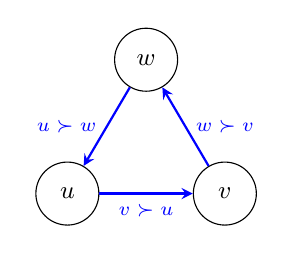
\begin{tikzpicture}[
    node/.style={circle, draw, minimum size=0.8cm, font=\small},
    arr/.style={->, >=stealth, thick, blue}
]
    \node[node] (u) at (0, 0) {$u$};
    \node[node] (v) at (2, 0) {$v$};
    \node[node] (w) at (1, 1.7) {$w$};
    \draw[arr] (u) -- (v) node[midway, below, font=\scriptsize] {$v \succ u$};
    \draw[arr] (v) -- (w) node[midway, right, font=\scriptsize] {$w \succ v$};
    \draw[arr] (w) -- (u) node[midway, left, font=\scriptsize] {$u \succ w$};
\end{tikzpicture}
\end{center}

Không mất tính tổng quát, thuật toán xác định $\mathcal{A}$ phải trả về một trong hai thứ hạng cho $\{u,v,w\}$:
\begin{itemize}
    \item \textbf{Trường hợp 1: $\mathcal{A}$ trả về $u, v, w$} (tức $u$ đứng đầu, $w$ đứng cuối). Chọn $\sigma^*$ đặt $w$ là điểm tích cực ($+$) và $u, v$ là tiêu cực ($-$). Khi đó:
    \begin{align*}
        L(h, \sigma^*) &= \frac{2}{3 \cdot 2}\bigl[h(u,w)\cdot 1 + h(v,w) \cdot 1\bigr] = \frac{1}{3}\bigl[0 + 0\bigr] + \frac{1}{3} h(u,w) = \frac{1}{3},
    \end{align*}
    cụ thể là $h$ nói $u \succ w$ (tức $h(u,w)=1$ trong ví dụ này), nhưng $\sigma^*$ xếp $w$ là dương. Nên $L(h, \sigma^*) = \frac{1}{3}$.
    
    Còn $\mathcal{A}$ xếp $u, v$ trên $w$, nhưng $w$ là dương, nên cả hai cặp $(u,w)$ và $(v,w)$ đều bị xếp sai. Do đó $L(\mathcal{A}, \sigma^*) = \frac{2}{3}$.
    
    \item \textbf{Trường hợp 2: $\mathcal{A}$ trả về $w, v, u$}. Chọn $\sigma^*$ đặt $u$ là dương, $w, v$ là tiêu cực. Tương tự, ta có $L(h, \sigma^*) = \frac{1}{3}$ và $L(\mathcal{A}, \sigma^*) = \frac{2}{3}$.
\end{itemize}

Trong cả hai trường hợp, $L(\mathcal{A}, \sigma^*) = 2 \cdot L(h, \sigma^*)$. Vì $\sigma^*$ tối ưu có thể đạt được (nếu $h$ được học hoàn hảo), ta có $\mathrm{Reg}(\mathcal{A}) \geq 2 \, \mathrm{Reg}(h)$.
\end{proof}

\begin{morong}
\textbf{Tại sao chu trình là thách thức của thuật toán xác định?}

Khi hàm ưu tiên $h$ cảm sinh chu trình (ví dụ $u \succ_h v \succ_h w \succ_h u$), một thuật toán xác định buộc phải "lựa chọn" một hướng cụ thể cho mỗi cặp. Chọn $u$ trước $v$ có thể tốt với một số $(X, \sigma^*)$, nhưng đối phương có thể chọn $\sigma^*$ sao cho lựa chọn này bị phạt. Ngẫu nhiên hóa tránh được hạn chế này bằng cách "đặt cược" theo xác suất $h(u,v)$, không cam kết hoàn toàn vào một hướng.
\end{morong}

% -------- 10.6.3 Randomized --------
\subsubsection{Thuật Toán Ngẫu Nhiên: QuickSort Dựa Trên Hàm Ưu Tiên}
\label{sec:quicksort_pref}

Kết quả về chặn dưới cho thấy cần dùng ngẫu nhiên hóa để vượt qua hệ số 2. Thuật toán đề xuất là phiên bản mở rộng của \textbf{QuickSort ngẫu nhiên}, trong đó hàm so sánh được thay bằng hàm ưu tiên $h$.

\paragraph{Mô tả thuật toán.}
Tại mỗi bước đệ quy, một phần tử \emph{pivot} $u$ được chọn đồng đều ngẫu nhiên từ $X$. Với mỗi phần tử còn lại $v \neq u$:
\begin{itemize}
    \item $v$ được đặt \textbf{bên trái} $u$ (xếp trước $u$) với xác suất $h(v, u)$,
    \item $v$ được đặt \textbf{bên phải} $u$ (xếp sau $u$) với xác suất $h(u, v) = 1 - h(v,u)$.
\end{itemize}
Thuật toán đệ quy trên mảng bên trái và bên phải, sau đó ghép nối kết quả.

\begin{figure}[H]
\centering
\begin{tikzpicture}[
    boxa/.style={draw, rounded corners=6pt, align=center,
                 minimum width=3.5cm, minimum height=1.1cm, font=\small},
    node distance=0pt
]
    \node[boxa, fill=yellow!25, draw=orange!60]
        (pivot) at (0,0)
        {\textbf{Pivot $u$} \\ \scriptsize chọn ngẫu nhiên từ $X$};

    \node[boxa, fill=teal!15, draw=teal!50]
        (left) at (-3.6,-3.0) {\textbf{Bên trái} \\ \scriptsize $\{v: h(v,u)>\text{rand}\}$};

    \node[boxa, fill=purple!12, draw=purple!40]
        (right) at (3.6,-3.0) {\textbf{Bên phải} \\ \scriptsize $\{v: h(u,v)>\text{rand}\}$};

    \node[boxa, fill=gray!10, draw=gray!40, minimum width=7.0cm]
        (result) at (0,-5.8)
        {\scriptsize Kết quả: [đệ quy trái] $+$ [$u$] $+$ [đệ quy phải]};

    % Diagonal arrows Pivot → Left/Right (straight lines touching box corners)
    \draw[->, >=stealth, thick]
        (pivot.south west) -- (left.north east)
        node[midway, above left, font=\scriptsize] {xác suất $h(v,u)$};

    \draw[->, >=stealth, thick]
        (pivot.south east) -- (right.north west)
        node[midway, above right, font=\scriptsize] {xác suất $h(u,v)$};

    % L-shape arrows Left/Right → Result
    \draw[->, >=stealth, thick]
        (left.south) -- ++(0,-0.55) -| ([xshift=-1.2cm]result.north);

    \draw[->, >=stealth, thick]
        (right.south) -- ++(0,-0.55) -| ([xshift=1.2cm]result.north);
\end{tikzpicture}
\caption{Thuật toán QuickSort ngẫu nhiên dựa trên hàm ưu tiên $h$.
Tính chất cốt lõi: $\Pr[\mathcal{A}_{\mathrm{QS}} \text{ xếp } u \text{ trước } v] = h(u,v)$,
dẫn đến mất mát kỳ vọng bằng đúng $L(h, \sigma^*)$ — không có hệ số nhân 2.}
\end{figure}

\begin{theorem}[Chặn hiệu năng cho QuickSort ngẫu nhiên -- Định lý 2.5 mở rộng]
\label{thm:quicksort_pref}
Ký hiệu $\mathcal{A}_{\mathrm{QS}}$ là thuật toán QuickSort ngẫu nhiên dùng hàm ưu tiên $h$. Trong cài đặt nhị phân:
\begin{align}
    \mathbb{E}_{X, \sigma^*, s}\bigl[L\bigl(\mathcal{A}_{\mathrm{QS}}(X, s), \sigma^*\bigr)\bigr] &= \mathbb{E}_{X, \sigma^*}\bigl[L(h, \sigma^*)\bigr], \label{eq:qs_loss} \\
    \mathrm{Reg}\bigl(\mathcal{A}_{\mathrm{QS}}\bigr) &\leq \mathrm{Reg}(h). \label{eq:qs_regret}
\end{align}
Hơn nữa, trong cài đặt tổng quát (không nhất thiết nhị phân):
\begin{equation}
    \mathbb{E}_{X, \sigma^*, s}\bigl[L\bigl(\mathcal{A}_{\mathrm{QS}}(X, s), \sigma^*\bigr)\bigr] \leq 2\, \mathbb{E}_{X, \sigma^*}\bigl[L(h, \sigma^*)\bigr]. \label{eq:qs_general}
\end{equation}
\end{theorem}

\begin{proof}[Ý tưởng chứng minh cho \eqref{eq:qs_loss}]
Chứng minh dựa trên phân tích kỳ vọng của mất mát cho từng cặp $(u,v)$. Với bất kỳ cặp $(u,v)$, thuật toán xếp $u$ trước $v$ khi:
\begin{itemize}
    \item $u$ là pivot và $v$ bị đưa sang phải (xác suất $h(u,v) \cdot \frac{2}{|X|}$), hoặc
    \item $v$ là pivot và $u$ ở bên trái (xác suất $h(u,v) \cdot \frac{2}{|X|}$), hoặc
    \item Một phần tử khác là pivot và hai bước đệ quy xử lý cặp này.
\end{itemize}

Bằng quy nạp cẩn thận, người ta chứng minh rằng \emph{kỳ vọng xác suất} của sự kiện ``$\mathcal{A}_{\mathrm{QS}}$ xếp $u$ trước $v$'' bằng chính xác $h(u,v)$. Nói cách khác:
\[
    \Pr_s[\mathcal{A}_{\mathrm{QS}} \text{ xếp } u \text{ trước } v] = h(u, v).
\]
Do đó:
\begin{align*}
    \mathbb{E}_s[L(\mathcal{A}_{\mathrm{QS}}, \sigma^*)] &= \frac{2}{n(n-1)} \sum_{u \neq v} \Pr_s[\mathcal{A}_{\mathrm{QS}} \text{ xếp } u \text{ trước } v] \cdot \mathbf{1}_{\sigma^*(v) < \sigma^*(u)} \\
    &= \frac{2}{n(n-1)} \sum_{u \neq v} h(u,v) \cdot \mathbf{1}_{\sigma^*(v) < \sigma^*(u)} = L(h, \sigma^*).
\end{align*}
Lấy kỳ vọng theo $(X, \sigma^*)$ ta được đẳng thức \eqref{eq:qs_loss}.
\end{proof}

\paragraph{Lợi ích của QuickSort ngẫu nhiên so với Sort-by-Degree.}
\begin{itemize}
    \item \textbf{Hệ số 2 biến mất:} Mất mát kỳ vọng \emph{bằng chính xác} mất mát của $h$, không phải gấp đôi.
    \item \textbf{Độ phức tạp tốt hơn:} Độ phức tạp thời gian kỳ vọng là $O(n \log n)$, so với $\Omega(n^2)$ của sort-by-degree.
    \item \textbf{Linh hoạt:} Nếu chỉ cần top-$k$ phần tử (như trong hầu hết ứng dụng thực tế), độ phức tạp giảm xuống $O(n + k \log k)$.
\end{itemize}

\begin{morong}
\textbf{Ưu thế của ngẫu nhiên hóa so với xác định.}

Thuật toán xác định (sort-by-degree) gặp hạn chế vì phải "cam kết" lựa chọn vị trí cho mỗi cặp. Khi hàm $h$ có chu trình, lựa chọn này luôn gây lỗi hệ thống với hệ số nhân 2.

Thuật toán ngẫu nhiên (QuickSort) tránh được bẫy này bằng cách phân phối xác suất xếp sai mỗi cặp bằng chính xác $h(u,v)$ -- là một \emph{unbiased estimator} của hàm ưu tiên. Kết quả: không có thêm lỗi nào so với chất lượng của $h$ bản thân.
\end{morong}

% -------- 10.6.4 Extension --------
\subsubsection{Mở Rộng Sang Các Hàm Mất Mát Có Trọng Số}

\begin{definition}[Hàm mất mát có trọng số $L_\omega$]
Tất cả các kết quả trên có thể mở rộng cho lớp tổng quát các hàm mất mát $L_\omega$ được định nghĩa bởi hàm trọng số (emphasis function) $\omega: \mathbb{N} \times \mathbb{N} \to \mathbb{R}^+$:
\begin{equation}
    L_\omega(\sigma, \sigma^*) = \frac{2}{n(n-1)} \sum_{u \neq v} \omega(\sigma^*(v), \sigma^*(u))\, \mathbf{1}_{\sigma(u) < \sigma(v)}\, \mathbf{1}_{\sigma^*(v) < \sigma^*(u)}.
    \label{eq:loss_omega}
\end{equation}
\end{definition}

Hàm $\omega$ phải thỏa mãn ba tiên đề:
\begin{enumerate}
    \item \textbf{Tính đối xứng:} $\omega(i,j) = \omega(j,i)$ với mọi $i, j$.
    \item \textbf{Tính đơn điệu:} $\omega(i,j) \leq \omega(i,k)$ nếu $i < j < k$ hoặc $i > j > k$ (lỗi ở vị trí xa nhau bị phạt nặng hơn).
    \item \textbf{Bất đẳng thức tam giác:} $\omega(i,j) \leq \omega(i,k) + \omega(k,j)$.
\end{enumerate}

\paragraph{Các ví dụ quan trọng về $\omega$.}
\begin{itemize}
    \item $\omega(i,j) = 1$ với mọi $i \neq j$: thu về hàm mất mát chuẩn \eqref{eq:loss_pref}.
    \item $\omega(i,j) = \mathbf{1}_{(i \leq k) \vee (j \leq k)}$ (cho $k$ cố định): nhấn mạnh lỗi ở top-$k$. Mọi sai lệch liên quan đến ít nhất một phần tử trong top-$k$ đều bị phạt. Dùng cho ứng dụng search engine khi chỉ quan tâm top-$k$ kết quả.
    \item $\omega(i,j) = \frac{n(n-1)}{2m^+m^-}$ (trong bipartite với $m^+$ điểm dương, $m^-$ điểm âm): thu về hàm mất mát tương đương $1 - \mathrm{AUC}$.
\end{itemize}

% ============================================================
\subsection{Các Tiêu Chí Xếp Hạng Khác (Other Ranking Criteria)}
\label{sec:other_ranking}
% ============================================================

Các phần trước dựa hoàn toàn trên sai số theo cặp (pairwise misranking). Trong thực tế, đặc biệt là trong \emph{truy xuất thông tin} (information retrieval) và các hệ thống search engine, nhiều tiêu chí khác cũng được sử dụng rộng rãi. Phần này trình bày hệ thống các tiêu chí này.

% -------- Precision / Recall --------
\subsubsection{Precision, Recall và Average Precision}

\paragraph{Thiết lập chung.}
Các tiêu chí này giả định dữ liệu được phân thành hai lớp: \emph{điểm dương} (liên quan, relevant) và \emph{điểm âm} (không liên quan, irrelevant). Cho một hàm xếp hạng $h$, ta xếp các điểm theo thứ tự điểm số giảm dần và xét top-$n$ kết quả.

\begin{definition}[Precision và Recall]
Gọi $R^+$ là tập tất cả điểm dương, $P_n$ là tập top-$n$ điểm được xếp cao nhất bởi $h$.
\begin{align}
    \mathrm{Precision}(h) &= \frac{|P \cap R^+|}{|P|} \quad (\text{trong đó } P = P_{|P|}), \label{eq:precision}\\
    \mathrm{Precision@n}(h) &= \frac{|P_n \cap R^+|}{n}, \label{eq:precision_at_n}\\
    \mathrm{Recall}(h) &= \frac{|P \cap R^+|}{|R^+|}. \label{eq:recall}
\end{align}
\end{definition}

\textbf{Giải thích:}
\begin{itemize}
    \item \textbf{Precision} (độ chính xác): trong các điểm được dự đoán là dương, có bao nhiêu phần trăm thực sự dương?
    \item \textbf{Precision@$n$}: trong top-$n$ kết quả trả về, có bao nhiêu phần trăm là dương?
    \item \textbf{Recall} (độ phủ): trong tất cả điểm dương thực sự, có bao nhiêu phần trăm được dự đoán đúng là dương?
\end{itemize}

\begin{example}[Tính Precision@$k$ cho search engine]
Giả sử có 10 tài liệu liên quan ($|R^+| = 10$) trong cơ sở dữ liệu 100 tài liệu. Hệ thống trả về top-5 tài liệu, trong đó 4 tài liệu liên quan.

\begin{align*}
    \mathrm{Precision@5} &= \frac{4}{5} = 0.8 = 80\%, \\
    \mathrm{Recall}(\text{top-5}) &= \frac{4}{10} = 0.4 = 40\%.
\end{align*}

Nếu top-10 được trả về với 8 tài liệu liên quan:
\begin{align*}
    \mathrm{Precision@10} &= \frac{8}{10} = 0.8, \quad \mathrm{Recall}(\text{top-10}) = \frac{8}{10} = 0.8.
\end{align*}
\end{example}

\paragraph{Average Precision (AP).}
Một vấn đề của Precision@$n$ là nó chỉ đo tại \emph{một ngưỡng cố định}. Average Precision (AP) tổng hợp thông tin ở \emph{tất cả các ngưỡng}:

\begin{definition}[Average Precision]
\begin{equation}
    \mathrm{AP}(h) = \frac{1}{|R^+|} \sum_{n=1}^{N} \mathrm{Precision@n}(h) \cdot \mathbf{1}_{x_n \in R^+},
    \label{eq:ap}
\end{equation}
trong đó $x_n$ là tài liệu ở vị trí thứ $n$ trong thứ hạng của $h$, và $N$ là tổng số tài liệu. (Chỉ tính Precision@$n$ khi vị trí $n$ là một điểm dương.)
\end{definition}

\begin{example}[Tính Average Precision]
Giả sử có 4 tài liệu dương ($|R^+| = 4$) trong 8 tài liệu. Thứ hạng của $h$: $[+, -, +, +, -, -, +, -]$ (dấu $+$ là dương, $-$ là âm).

Tính Precision@$n$ tại các vị trí dương ($n = 1, 3, 4, 7$):
\begin{align*}
    \mathrm{P@1} &= 1/1 = 1.0, \quad \mathrm{P@3} = 2/3 \approx 0.667, \\
    \mathrm{P@4} &= 3/4 = 0.75, \quad \mathrm{P@7} = 4/7 \approx 0.571.
\end{align*}

\[
    \mathrm{AP}(h) = \frac{1}{4}(1.0 + 0.667 + 0.75 + 0.571) = \frac{2.988}{4} \approx 0.747.
\]
AP cao (0.747) phản ánh rằng các tài liệu dương được xếp ở vị trí cao.
\end{example}

\paragraph{Ưu và nhược điểm.}
\begin{itemize}
    \item \textbf{Ưu:} Dễ hiểu, trực tiếp phản ánh chất lượng top-$k$ kết quả. Precision@$n$ được dùng rộng rãi trong đánh giá search engine thực tế.
    \item \textbf{Nhược:} Precision@$n$ không xem xét thứ tự \emph{bên trong} top-$n$. AP nhạy cảm với kích thước $|R^+|$.
\end{itemize}

% -------- DCG / NDCG --------
\subsubsection{DCG và NDCG}
\label{sec:dcg_ndcg}

\paragraph{Động lực.}
Trong nhiều ứng dụng thực tế (ví dụ: xếp hạng sản phẩm thương mại điện tử), mỗi điểm có \emph{nhiều mức độ liên quan} khác nhau (không chỉ nhị phân liên quan/không liên quan). Tiêu chí DCG/NDCG được thiết kế để xử lý trường hợp này.

\begin{definition}[Discounted Cumulative Gain (DCG)]
Cho chuỗi hệ số chiết khấu không tăng $c_1 \geq c_2 \geq \cdots \geq 0$ (ví dụ $c_i = \log_2(i+1)^{-1} = \frac{1}{\log_2(i+1)}$). Cho một thứ hạng $\sigma$ với điểm liên quan $r_i$ tại vị trí thứ $i$:
\begin{equation}
    \mathrm{DCG}(\sigma) = \sum_{i=1}^{m} c_i \cdot r_i.
    \label{eq:dcg}
\end{equation}
\end{definition}

\textbf{Trực giác:} Tài liệu ở vị trí càng cao (index $i$ nhỏ) nhận trọng số $c_i$ lớn hơn, phản ánh thực tế người dùng ít có khả năng xem kết quả ở trang 2, 3, $\ldots$ Tài liệu liên quan $r_i$ lớn (rất liên quan) ở vị trí đầu đóng góp nhiều vào DCG.

\begin{definition}[Normalized DCG (NDCG)]
\begin{equation}
    \mathrm{NDCG}(\sigma) = \frac{\mathrm{DCG}(\sigma)}{\mathrm{IDCG}},
    \label{eq:ndcg}
\end{equation}
trong đó $\mathrm{IDCG}$ (Ideal DCG) là DCG của thứ hạng \emph{hoàn hảo} --- sắp xếp các tài liệu theo điểm liên quan giảm dần:
\begin{equation}
    \mathrm{IDCG} = \sum_{i=1}^{m} c_i \cdot r^*_i, \quad r^*_1 \geq r^*_2 \geq \cdots \geq r^*_m.
    \label{eq:idcg}
\end{equation}
\end{definition}

NDCG luôn nằm trong $[0, 1]$. Giá trị NDCG = 1 nghĩa là thứ hạng dự đoán hoàn toàn khớp với thứ hạng lý tưởng.

\begin{example}[Tính DCG và NDCG bằng tay]
Cho 5 tài liệu với điểm liên quan $[r_1, r_2, r_3, r_4, r_5] = [3, 2, 0, 1, 0]$ (tương ứng thứ hạng của hệ thống) và hệ số chiết khấu $c_i = \frac{1}{\log_2(i+1)}$:

\begin{align*}
    c_1 = \frac{1}{\log_2 2} = 1, \quad c_2 = \frac{1}{\log_2 3} \approx 0.631, \quad c_3 = \frac{1}{\log_2 4} = 0.5, \\
    c_4 = \frac{1}{\log_2 5} \approx 0.431, \quad c_5 = \frac{1}{\log_2 6} \approx 0.387.
\end{align*}

\[
    \mathrm{DCG} = 1 \cdot 3 + 0.631 \cdot 2 + 0.5 \cdot 0 + 0.431 \cdot 1 + 0.387 \cdot 0 \approx 3 + 1.262 + 0 + 0.431 = 4.693.
\]

Thứ hạng lý tưởng: $[3, 2, 1, 0, 0]$:
\[
    \mathrm{IDCG} = 1 \cdot 3 + 0.631 \cdot 2 + 0.5 \cdot 1 + 0.431 \cdot 0 + 0.387 \cdot 0 = 3 + 1.262 + 0.5 = 4.762.
\]

\[
    \mathrm{NDCG} = \frac{4.693}{4.762} \approx 0.985.
\]

Giá trị NDCG cao (0.985) cho thấy thứ hạng dự đoán rất gần với thứ hạng lý tưởng: tài liệu có điểm liên quan cao nhất ($r=3$) được đặt đúng ở vị trí đầu, tài liệu $r=1$ chỉ bị dịch xuống một bậc.
\end{example}

\begin{figure}[H]
\centering
\begin{tikzpicture}[scale=0.9]
    \def\barw{0.65}
    \def\gap{0.2}
    % Axes
    \draw[->] (-0.3,0) -- (10.0,0) node[right,font=\small] {Vị trí $i$};
    \draw[->] (0,-0.1) -- (0,3.6) node[above,font=\small] {$r_i$, $3 \cdot c_i$};

    % Tick marks and labels on y-axis
    \foreach \y/\lab in {1/1, 2/2, 3/3} {
        \draw (-0.08,\y) -- (0.08,\y);
        \node[left,font=\scriptsize] at (-0.05,\y) {\lab};
    }

    % Bars: positions 1..5 centered at x = 1.3, 3.0, 4.7, 6.4, 8.1
    \def\xone{1.30}
    \def\xtwo{3.00}
    \def\xthree{4.70}
    \def\xfour{6.40}
    \def\xfive{8.10}

    % Bar 1: r=3
    \fill[blue!55, opacity=0.85]
        (\xone-\barw/2, 0) rectangle (\xone+\barw/2, 3);
    \draw[blue!70] (\xone-\barw/2, 0) rectangle (\xone+\barw/2, 3);
    \node[white, font=\scriptsize\bfseries] at (\xone, 2.5) {$r{=}3$};

    % Bar 2: r=2
    \fill[blue!45, opacity=0.75]
        (\xtwo-\barw/2, 0) rectangle (\xtwo+\barw/2, 2);
    \draw[blue!60] (\xtwo-\barw/2, 0) rectangle (\xtwo+\barw/2, 2);
    \node[white, font=\scriptsize\bfseries] at (\xtwo, 1.5) {$r{=}2$};

    % Bar 3: r=0 (empty, just axis tick)
    % Bar 4: r=1
    \fill[blue!30, opacity=0.65]
        (\xfour-\barw/2, 0) rectangle (\xfour+\barw/2, 1);
    \draw[blue!45] (\xfour-\barw/2, 0) rectangle (\xfour+\barw/2, 1);
    \node[blue!80, font=\scriptsize\bfseries] at (\xfour, 0.5) {$r{=}1$};

    % Bar 5: r=0 (empty)

    % X-axis labels
    \foreach \x/\lab in {\xone/1, \xtwo/2, \xthree/3, \xfour/4, \xfive/5} {
        \draw (\x, -0.07) -- (\x, 0.07);
        \node[below, font=\scriptsize] at (\x, -0.05) {Vị trí $\lab$};
    }

    % Discount curve c_i = 1/log2(i+1):
    %   c1 = 1.0   -> (\xone,  1.0) -- top of bar 1? No, we scale to data coords.
    %   We want c_i drawn in the same y-scale as r.
    %   c1=1.0, c2≈0.631, c3=0.5, c4≈0.431, c5≈0.387
    %   Multiply by 3 so c1 starts at y=3.0 (top of bar 1)
    %   c1=3.0, c2≈1.893, c3=1.5, c4≈1.292, c5≈1.161
    \draw[red!70, thick, dashed]
        (\xone,  3.000) ..controls (\xone+0.3, 3.0) and (\xtwo-0.3, 1.893)..
        (\xtwo,  1.893) ..controls (\xtwo+0.3, 1.893) and (\xthree-0.3, 1.5)..
        (\xthree,1.500) ..controls (\xthree+0.3,1.5) and (\xfour-0.3, 1.292)..
        (\xfour, 1.292) ..controls (\xfour+0.3, 1.292) and (\xfive-0.3, 1.161)..
        (\xfive, 1.161);

    % Endpoint label
    \node[red!70, right, font=\small] at (\xfive+0.05, 1.161) {$c_i$};

    % Legend
    \fill[blue!45, opacity=0.75] (4.6, 3.2) rectangle (5.0, 3.5);
    \node[right, font=\scriptsize] at (5.05, 3.35) {Điểm liên quan $r_i$};
    \draw[red!70, thick, dashed] (4.6, 2.8) -- (5.0, 2.8);
    \node[right, font=\scriptsize] at (5.05, 2.8) {Hệ số chiết khấu $c_i$};
\end{tikzpicture}
\caption{Minh họa DCG: cột màu xanh là điểm liên quan $r_i$ tại mỗi vị trí,
đường đỏ nét đứt là hệ số chiết khấu $c_i = \frac{1}{\log_2(i+1)}$ giảm dần,
bắt đầu từ $c_1 = 1.0$ (đỉnh cột đầu tiên). DCG là tổng tích $c_i \cdot r_i$.}
\label{fig:dcg_visual}
\end{figure}

\paragraph{Ưu và nhược điểm của DCG/NDCG.}
\begin{itemize}
    \item \textbf{Ưu:} Xử lý được nhiều mức độ liên quan; chiết khấu theo vị trí phản ánh hành vi thực tế của người dùng; NDCG chuẩn hóa cho phép so sánh giữa các truy vấn khác nhau.
    \item \textbf{Nhược:} Tính toán phức tạp hơn precision; kết quả phụ thuộc vào lựa chọn hàm chiết khấu $c_i$; không có dạng đóng (closed form) cho bài toán tối ưu.
\end{itemize}

% -------- Mối liên hệ --------
\subsubsection{Mối Liên Hệ Giữa Các Tiêu Chí và Với AUC}
\label{sec:criteria_connections}

\begin{morong}

% \textbf{Bảng so sánh toàn diện các tiêu chí xếp hạng}
% \begin{table}[H]
% \centering
% \small
% \begin{tabular}{|c|c|c|c|c|}
% \hline
% \textbf{Tiêu chí} & \textbf{Nhãn yêu cầu} & \textbf{Phạm vi} & \textbf{Nhấn mạnh} & \textbf{Ứng dụng điển hình} \\
% \hline
% Pairwise error & Nhị phân / thứ hạng & $[0,1]$ & Toàn bộ cặp & Lý thuyết học máy \\
% \hline
% AUC & Nhị phân & $[0,1]$ & Tổng thể, mọi ngưỡng & Phân loại y tế, fraud \\
% \hline
% Precision@$k$ & Nhị phân & $[0,1]$ & Top-$k$ chính xác & Search engine \\
% \hline
% Average Precision & Nhị phân & $[0,1]$ & Vị trí các điểm dương & IR đánh giá hệ thống \\
% \hline
% DCG / NDCG & Thứ tự liên quan & $[0,1]$ & Liên quan + vị trí & Web search, khuyến nghị \\
% \hline
% \end{tabular}
% \caption{So sánh các tiêu chí xếp hạng trong học máy và truy xuất thông tin.}
% \label{tab:criteria_comparison}
% \end{table}

\textbf{Mối liên hệ toán học giữa AUC và pairwise error} đã được phân tích trong Mục~\ref{sec:bipartite}: $\mathrm{AUC} = 1 - R(h)$.

\textbf{Liên hệ giữa Precision@$k$ và $L_\omega$:} Như đã trình bày trong Mục~\ref{sec:other_ranking}, bằng cách chọn $\omega(i,j) = \mathbf{1}_{(i \leq k) \vee (j \leq k)}$, hàm mất mát $L_\omega$ trở thành một proxy cho precision@$k$ trong khuôn khổ preference-based.

\textbf{Liên hệ giữa Average Precision và MAP (Mean Average Precision):} MAP là trung bình của AP trên nhiều truy vấn:
\begin{equation}
    \mathrm{MAP} = \frac{1}{Q}\sum_{q=1}^{Q} \mathrm{AP}(h, q),
    \label{eq:map}
\end{equation}
trong đó $Q$ là số truy vấn. MAP là tiêu chí chuẩn để đánh giá hệ thống search engine.

\textbf{Hạn chế của AUC mà các tiêu chí khác bổ sung:} AUC tính trung bình trên \emph{toàn bộ} đường ROC -- nó không phân biệt giữa hệ thống tốt ở vùng FPR thấp (quan trọng trong fraud detection) và hệ thống tốt ở vùng FPR cao. Partial AUC, Precision@$k$ và NDCG giải quyết hạn chế này bằng cách tập trung vào vùng quan tâm.
\end{morong}

% -------- Liên hệ chương khác --------
\subsubsection{Mối Liên Hệ Giữa Preference-Based Setting Và Các Phần Khác}

\paragraph{Liên hệ với Score-based Setting.}
Score-based và preference-based là hai góc nhìn bổ trợ nhau:
\begin{itemize}
    \item Mọi hàm scoring $f: \mathcal{X} \to \mathbb{R}$ đều cảm sinh một hàm ưu tiên bắc cầu $h_f(u,v) = \mathbf{1}_{f(u) > f(v)} + \frac{1}{2}\mathbf{1}_{f(u)=f(v)}$.
    \item Ngược lại, từ hàm ưu tiên $h$ nhất quán theo cặp, có thể xây dựng hàm scoring gần đúng bằng sort-by-degree hoặc QuickSort.
    \item Hạn chế cơ bản: score-based \emph{bắt buộc} bắc cầu; preference-based \emph{không yêu cầu} tính chất này.
\end{itemize}

\paragraph{Liên hệ với RankBoost.}
RankBoost tối ưu hóa hàm mất mát pairwise exponential, kết quả là một \emph{hàm scoring} $f = \sum_t \alpha_t h_t$. Khi dùng trong preference-based, kết quả của RankBoost giai đoạn 1 cần được chuyển sang hàm ưu tiên: $h(u,v) = \sigma(f(u) - f(v))$ (hàm sigmoid). Điểm khác biệt là RankBoost tối ưu toàn cục trên không gian $\mathcal{X}$, trong khi preference-based chỉ cần chính xác trên tập con truy vấn $X$.

\paragraph{Liên hệ với Bipartite Ranking.}
Cài đặt nhị phân (bipartite) là trường hợp đặc biệt của cả score-based lẫn preference-based. Trong cài đặt này:
\begin{itemize}
    \item Hàm mất mát $L_\omega$ với $\omega(i,j) = \frac{n(n-1)}{2m^+m^-}$ thu về $1 - \mathrm{AUC}$.
    \item Các chặn của sort-by-degree (hệ số 2) và QuickSort (hệ số 1) đều được chứng minh trong cài đặt nhị phân, sau đó tổng quát hóa.
\end{itemize}

\paragraph{Liên hệ với lý thuyết tổng quát hóa -- Rademacher Complexity (Chương 3).}
Mặc dù phần preference-based setting không trình bày chặn tổng quát hóa theo Rademacher complexity một cách tường minh (vì khuôn khổ regret đã đủ), sự liên hệ ngầm vẫn tồn tại: chất lượng của hàm ưu tiên $h$ ở giai đoạn 1 (học từ dữ liệu) được đảm bảo bởi các chặn generalization của Chương 3 và Theorem 10.1. Regret của giai đoạn 2 sau đó được kiểm soát thông qua regret của $h$ như trong section 10.6.2 và theorem 10.5.

% -------- Tóm tắt --------
% \subsubsection{Tóm Tắt Phần Preference-Based Setting}

% \begin{tcolorbox}[colback=blue!5, colframe=blue!60!black, title={\textbf{Điểm cốt lõi của Preference-Based Setting}}]
% \begin{enumerate}
%     \item \textbf{Hai giai đoạn:} Học hàm ưu tiên $h$ (từ dữ liệu) $\to$ Sinh thứ hạng (trên tập truy vấn). Tách biệt hoàn toàn, giúp dùng bất kỳ classifier nào ở giai đoạn 1.
    
%     \item \textbf{Không cần bắc cầu:} $h$ có thể không bắc cầu, phù hợp với preference thực tế của con người. Đây là ưu điểm cốt lõi so với score-based.
    
%     \item \textbf{Sort-by-degree:} Hệ số 2, độ phức tạp $\Omega(n^2)$. Theorem 10.5 chứng minh không thể cải thiện hệ số này với thuật toán xác định.
    
%     \item \textbf{QuickSort ngẫu nhiên:} Loại bỏ hoàn toàn hệ số 2, đạt $\mathrm{Reg}(\mathcal{A}_{\mathrm{QS}}) \leq \mathrm{Reg}(h)$. Độ phức tạp $O(n \log n)$ hoặc $O(n + k \log k)$ cho top-$k$.
    
%     \item \textbf{Kết luận:} Ngẫu nhiên hóa là \emph{cần thiết và đủ} để đạt được hệ số 1 trong bài toán preference-based ranking.
% \end{enumerate}
% \end{tcolorbox}

\vspace{0.5cm}